\chapter{Conclusions}
\label{chap:Conclusions}

%Summary: summarize work and impact, describe directions for further work, describe how this provides a framework for an end to end solution in radio astronomy as well as other domain specific applications
%Goal: show everything worked and was awesome
%State: needs results, should be quick to write but difficult to write now

%TODO: explain this in text
This dissertation presents an end to end solution that allows domain experts to take a high level idea and and translate it into a design indicating what types of hardware should be used to implement the instrument. 
The ORCAS tool is able to generate these designs quickly, making it a useful tool to explore the design space of different astronomy algorithms.
I demonstrate three types of instrument design, and explore how changing the parameters affects the implementation and costs of these instruments.

In the results, it is clear that this approach is much quicker than designing instruments by hand. 
The ORCAS flow is able to map small designs in a few seconds and larger designs still take less than an hour to map.
Coupled with optimization techniques that reduce the number of blocks that need to be placed, ORCAS provides a scalable solution for mapping large instruments.
By allowing the user to leverage existing benchmarks, ORCAS reduces a traditional design cycle of a least a week down to an hour.
Furthermore, ORCAS provides a better design experience than the traditional approach.
The quick feedback is a key strength of this work, allowing the astronomer to vary the parameters of the algorithm and see how it affects the total cost.

Even when a benchmark isn't available, ORCAS makes it easy to add an estimated benchmark based on an existing one.
To get more accurate results, getting new data for a single benchmark is very fast.
The GPU benchmarks can be run in a few minutes and an FPGA benchmark for a small block can get results in under an hour.
So even if new benchmark data is needed, the entire design cycle will still take less than a day.

\section{Future Work}
The success of this work opens up a lot of related projects to improve upon the existing mapping capabilities.
While the instruments developed with ORCAS are designed for radio astronomy, ORCAS was developed as a general purpose tool and the expansion of the instrument set into other fields would provide interesting new challenges.
The existence of a DSP library and benchmarks would make it easy to transition to other DSP applications.

%Design interconenct
Since other applications might not need a full-crossbar network, it would also be useful to integrate network design into the ILP.
In radio astronomy, it is reasonable to assume this network exists and ignore the cost when designing instruments.
The toolflow currently allows the user to minimize the number of ports required but this still assumes the presence of a full-crossbar interconnect.
In applications with different network architectures, the costs can significantly change with the network design as well as the platforms used; future versions of this tool that are used for these applications will need to take those costs into account.


There are also improvements that can be made to the model, but they need to be balanced with the ILP to ensure fast runtimes.
As telescope arrays get larger, a single computational block may need to span multiple boards.
As we saw in the FX Correlator case study, this is going to be the case for the X-Engine in the near future.
Simply supporting that capability would be useful, but it would be better if the model was able to determine how to split these blocks between boards.

%Do a better job of preserving symmetry
Finally, the ILP aims to reduce cost in any way possible and often does so by cramming unrelated blocks onto the same platform.
ORCAS does support an option that forces the tool to create exactly one design on each platform, but this does not prevent the tool from putting unrelated blocks in the same design.
To make the resulting designs more straightforward, it would be useful if the ILP could preserve the problem structure when translating the design to hardware.


%\section{Final Conclusions}
%This work is a major step towards a universal clustered radio astronomy architecture.
%Figure \ref{fig: C5/universal_arch.png} gives an example of what this type of architecture could look like.
%
%
%\begin{figure}[ht!]
%  \centering
%    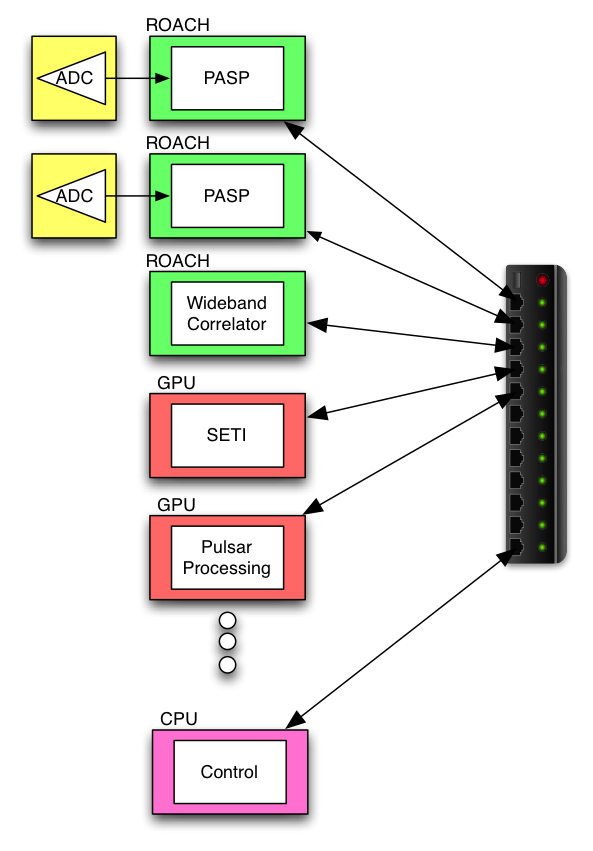
\includegraphics[width=0.5\textwidth]{Images/C5/universal_arch.png}
%  \caption{A potential architecture for multiple scientific instruments simultaneously processing data from the same telescope}
%  \label{fig: C5/universal_arch.png}
%\end{figure}
